\section{Accepttest}
\label{forforstaerker_accepttest}

Kravene specifikt til forforstærkeren er opstillet i tabel \ref{tab:krav_forforstaerker} og med henblik på at teste dem, er der udført målinger som beskrevet i Appendiks \ref{maaleforforstaerker}. Indgangsimpedansen er, som vist i tabel \ref{tab:resultatimpedans_forforstaerker}, med målingerne beregnet til 22,1 k\ohm~. Kravet lyder på 22 k\ohm, hvilket dermed ikke umiddelbart er opnået. Dog kan tolerancen på referencemodstanden alene, på 1 \%, som det ses i udregningen i formel (\ref{equ:forforstaerker_ztolerance}), være skyld i dette.

\begin{equation}
\label{equ:forforstaerker_ztolerance}
\vert Z \vert = \frac{\mathrm{14,6~mV}}{\mathrm{6,6~mV}} \cdot \mathrm{10~k\ohm} \pm 1~\% =  \mathrm{22,1~k\ohm} \pm 221~\ohm
\end{equation}

Dette krav betragtes derfor som opfyldt, hvilket kravet om forvrængning også gør. Som det ses på figur \ref{fig:accepttest-thdresultat-forforstaerker} topper denne mellem 0,20 \% og 0,25 \% og kravet lyder på maksimalt 0,5 \%. Under simuleringerne fandtes en THD på 0,2 \%, dog antages forskellen at ligge i at ulineariteterne i transistorerne ikke er korrekt beskrevet i simuleringsmodellerne. 

\begin{figure}[h]
\centering
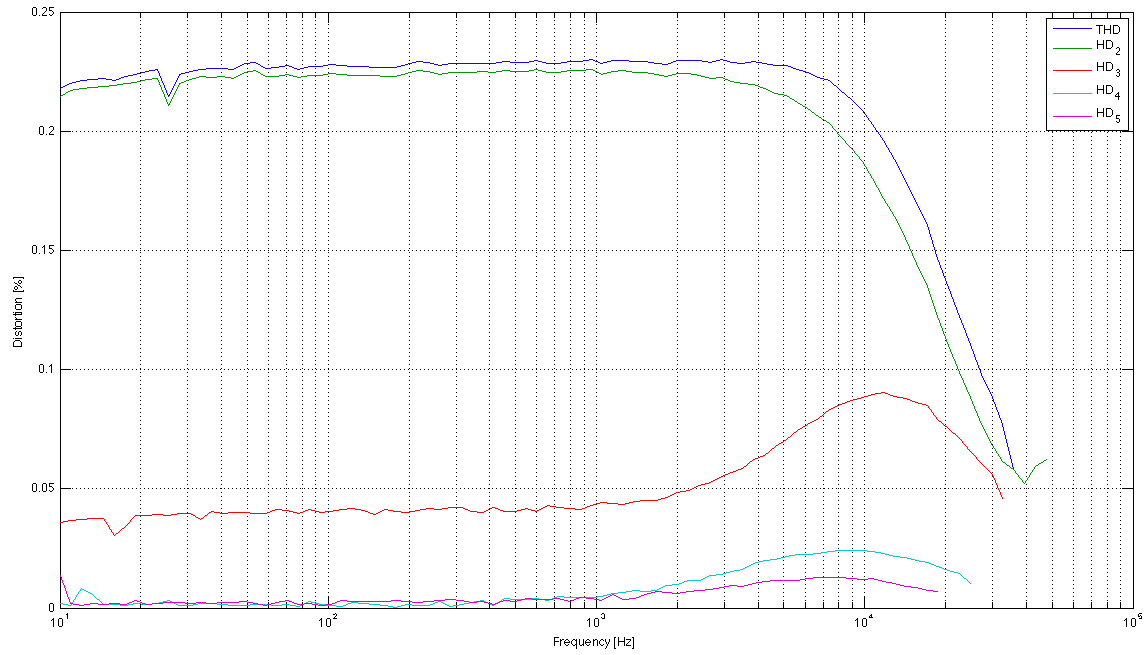
\includegraphics[scale=0.3]{maalerapporter/forforstaerker/thd-forforstaerker.png}
\caption{Forvrængningsmåleresultat for forforstærkeren}
\label{fig:accepttest-thdresultat-forforstaerker}
\end{figure}

\begin{figure}[h]
\centering
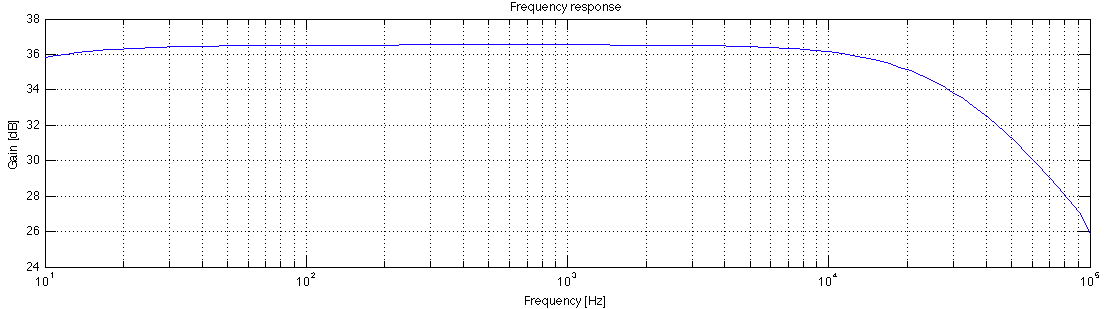
\includegraphics[width=\textwidth]{maalerapporter/forforstaerker/frekvensrespons-forforstaerker.png}
\caption{Frekvensgangs- og forstærkningsmåleresultater for forforstærkeren}
\label{fig:accepttest-fresultat-forforstaerker}
\end{figure}

Forstærkningen ved 1 kHz er, fra resultaterne afbilledet på figur \ref{fig:accepttest-fresultat-forforstaerker}, 36,54 dB, hvilket i udregningen vist i formel (\ref{equ:accepttest-forforstaerker-db-gange}) omregnes.

\begin{equation}
\label{equ:accepttest-forforstaerker-db-gange}
10^{\frac{\mathrm{36,54~dB}}{20}} = 67,1
\end{equation}

Dette opfylder ikke kravet på 69,7 gange, men resultaterne vurderes alligevel til at være gode. Forskellen tilskrives upræcis justering af potentiometre under implementeringen, hvilket også vurderes til at være årsagen til forskellen i forhold til simuleringen. 

\begin{figure}[h]
\centering
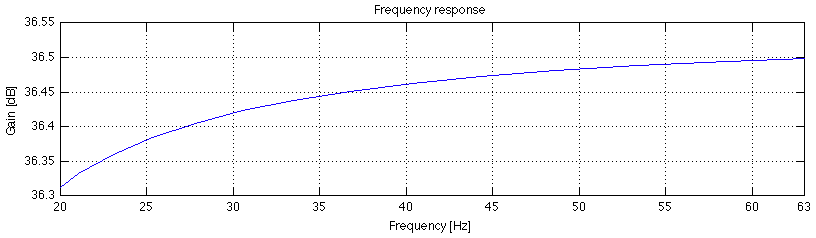
\includegraphics[width=\textwidth]{maalerapporter/forforstaerker/fr20-63.png}
\caption{Forforstærkerens målte frekvensgang fra 20 Hz til 63 Hz}
\label{fig:accepttest-fres-20-63}
\end{figure}

\begin{figure}[h]
\centering
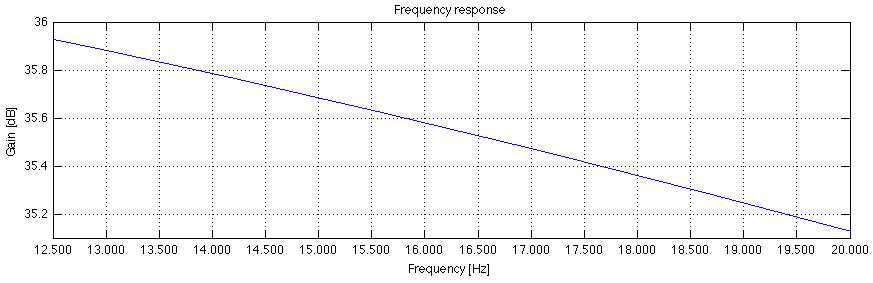
\includegraphics[width=\textwidth]{maalerapporter/forforstaerker/fr12-20k.png}
\caption{Forforstærkerens målte frekvensgangsresultater fra 12,5 kHz til 20 kHz}
\label{fig:accepttest-fres-125-20}
\end{figure}

Frekvensgangskravene er, som det kan ses på figur \ref{fig:accepttest-fresultat-forforstaerker}, figur \ref{fig:accepttest-fres-20-63} og figur \ref{fig:accepttest-fres-125-20}, opfyldt pånær kravet ved 12,5 kHz til 20 kHz, hvor den falder 0,8 dB. Dog udgør måleudstyret en kapacitiv belastning, som vist på figur \ref{fig:cap-error-diagram}, på 217 pF og coax-kablet der bruges udgør 101 pF i kapacitiv belastning \cite{maaling-mm5}.%\kilde{Ole Kiel Jensen, mm5 Måleteknik}. 

\begin{figure}[h]
\centering
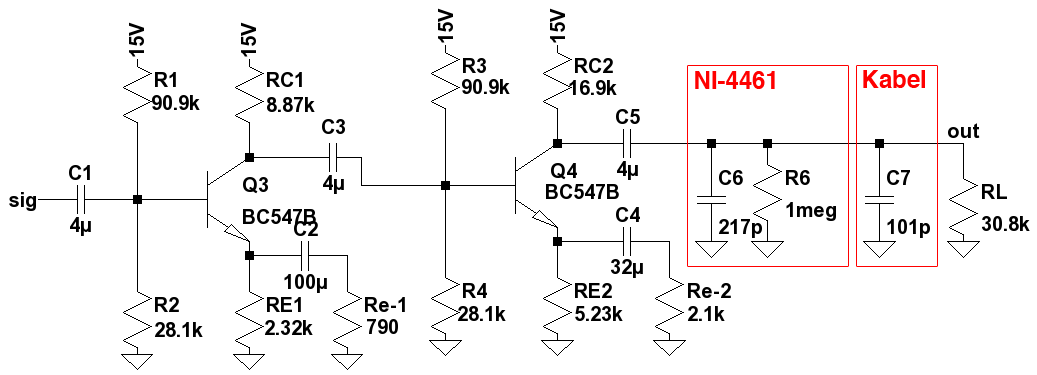
\includegraphics[scale=0.35]{teknisk/forforstaerker/cap-error-diagram.png}
\caption{Forforstærkerdiagram med kapacitiv belastning fra måleudstyr}
\label{fig:cap-error-diagram}
\end{figure}

Belastningen er et lavpasfilter, hvilket viser sig tydeligt ved simulering af forforstærkeren med denne belastning, som det kan ses på figur \ref{fig:cap-error}. Alene i simuleringen betyder denne belastning et fald på omkring 0,5 dB, hvormed selve forforstærkeren vurderes til at leve op til kravet. Derfor betragtes alle kravene til forforstærkeren som værende opfyldt.

\begin{figure}[h]
\centering
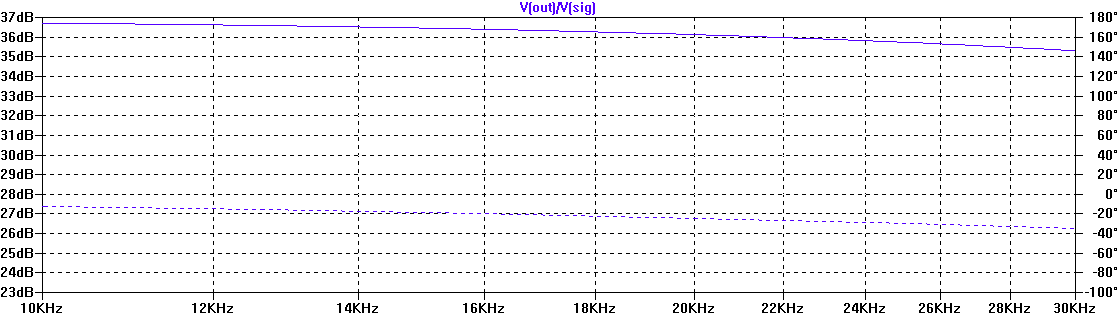
\includegraphics[width=\textwidth]{teknisk/forforstaerker/cap-error.png}
\caption{Simulering af forforstærkerens forstærkning med belastning fra måleudstyr}
\label{fig:cap-error}
\end{figure}